\chapter{Personal Area Networks \& Machine to machine Communication}
\label{sec:chapter5}

This chapter focuses on short-range wireless communication paradigms, including personal area networks (PANs) and machine to machine communications.


\section{Machine to machine communication}


Machine-to-machine (M2M) communication is the primary technology used for building  IoT frameworks \cite{MONTORI201856}. 
M2M encompasses the technologies that can be used in materializing the IoT network. Sensors, connectivity links, and radio interfaces form the critical components of M2M. M2M data collection networks help in collecting, managing, and analyzing the large chunk of device-generated data\cite{M2Mweb}. Typical M2M data collection networks include remote monitoring applications like asset tracking systems, inventory management systems, online energy meter reading, smart grid and homes, etc\cite{M2MAppli}. Quintessential M2M applications have simple hardware with sensors interfaced. Most of these devices are battery operated. Hence M2M mandates that the protocol used in communication to be simple and energy-efficient \cite{Survey1}.

\ac{lte} \ac{mtc} is an optimized version of LTE-Advanced (LTE-A) for M2M communication.  It introduces features like Enhanced Power Save Mode, Extended Discontinuous Reception, Longer sleep cycle, Connectionless Random Access Channel (RACH), and Less frequent Tracking Area Updates and measurements.
However, it has been shown that in typical Machine Type Communication (MTC) applications using  LTE based system, owing to the high device density and smaller size of the data packet, the signaling overhead will dominate, leading to lower resource utilization.   \cite{Ghavimi2015}. Further, the energy efficiency of the network will also be affected \cite{Gotsis2012}. Therefore 3GPP($3^{rd}$ generation partnership project) has proposed an architecture having a cluster of MTC devices under one cluster head to circumvent the issue mentioned above \cite{3GPP}. This type of cluster network is referred to as a data collection network. The cluster head often called the data collector (DC), facilitates the LTE-A base station to collect data from IoT devices  \cite{7159254}, \cite{Juan2013}. Data collection networks help in the efficient utilization of communication links and improve the throughput and energy efficiency of the M2M network \cite{Azari2015Scheduling}. For M2M data collection networks, DFSA has recently emerged to be a promising Medium Access Control(MAC)  protocol, \cite{Deng2010} \cite{Arun2}.

 Energy-efficient simple MAC protocols are crucial for the operation of M2M data collection networks \cite{7558142}. K. Langendoen et al. have presented a detailed survey on   low data rate MAC protocols for wireless sensor networks \cite{Langendoen:2010:AMP:1824766.1824775}.
Challenges in designing MAC protocol for an M2M-DC network are that the protocol should be able to handle a massive number of IoT nodes. 
Reservation based protocols like TDMA, FDMA, and CDMA have resource allocation overhead and are not efficient under dynamic load conditions such as M2M communication. Random access protocols based on ALOHA and carrier sense multiple access technique are less complex for incorporating low-cost IoT nodes. However, their throughput and energy efficiency get drastically reduced in large M2M networks due to high congestion.   


 For M2M networks under saturated traffic conditions, Frame Slotted Aloha (FSA)  is shown to be a promising protocol \cite{Survey1}.
 In FSA, $n$ nodes contend to transmit data to the DC over several frames. The number of frames in each slot is fixed, say to a value $m$. Each node selects uniformly at random one of the $m$ slots in the frame and transmits its data packet. The algorithm terminates when all nodes have successfully transmitted their data. In a Dynamic Frame Slotted Aloha (DFSA) based system, the number of slots $m$ in the frame is dynamically varied in each iteration to be equal to the number of contending nodes o as to provide the maximum throughput. Thus DFSA is dynamic, scalable, and well suited for massive IoT networks.
 
Variants of the FSA, such as Successive Interference Cancellation (SIC)-FSA, Reservation FSA (RFSA), Irregular Repeated Slotted Aloha(IRSA), and  Contention Resolution Diversity Slotted
Aloha (CRDSA), have been proposed as efficient medium access protocols for large M2M networks with saturated traffic conditions \cite{Survey1}.

Protocols based on FSA have been proposed for Wireless Sensor Networks (WSN) and in tag collision arbitration protocols applied to \ac{rfid} technology. \cite{Arun1} deals with the performance analysis of MPR-FSA, wherein the optimum MPR threshold that maximizes the throughput has been derived. It was shown that maximum throughput is achieved in FSA  when the number of slots available in a frame is the same as that of the number of contending devices. This idea has been implemented in the DFSA. 
Simulation studies of FSA and DFSA for class 0,1 RFID tag resolution protocols have been carried out \cite{Yan}. 
\cite{Deng2010} derived the optimum frame length that reduces the probability of collision among tags. Issues related to improving the probability of tag identification of a DFSA protocol used in the RFID system has been investigated in  \cite{Alcaraz}.

\subsection{MPR-DFSA MAC Protocol}

MPR DFSA MAC protocol works as follows. Assume $n$ as the total number of nodes in the DC domain. The DC estimates the value of $n$ and keeps track of it, using one of the well-known algorithms available in the literature, such as as\cite{Pudasaini}. 

  The DC uses Data Collection Rounds (DCRs) to periodically collect data from the different nodes, as illustrated in Fig.\ref{FigMPRDFSA}.DC sends a Request for Data (RFD) packet to initiate a DCR.  Following RFD, there will be several Data Collection Frames (DCFs). Each DCF consists of a varying number of slots. Slot length is the same as packet transmission duration. 
 The length of the DCF in units of slots ( $ = \lceil n \beta_K \rceil $ ) is announced by the RFD.  Each node transmits its data in the following DCFs, as explained below until it becomes successful. 
 
 \begin{figure}[h!]
  \centering
      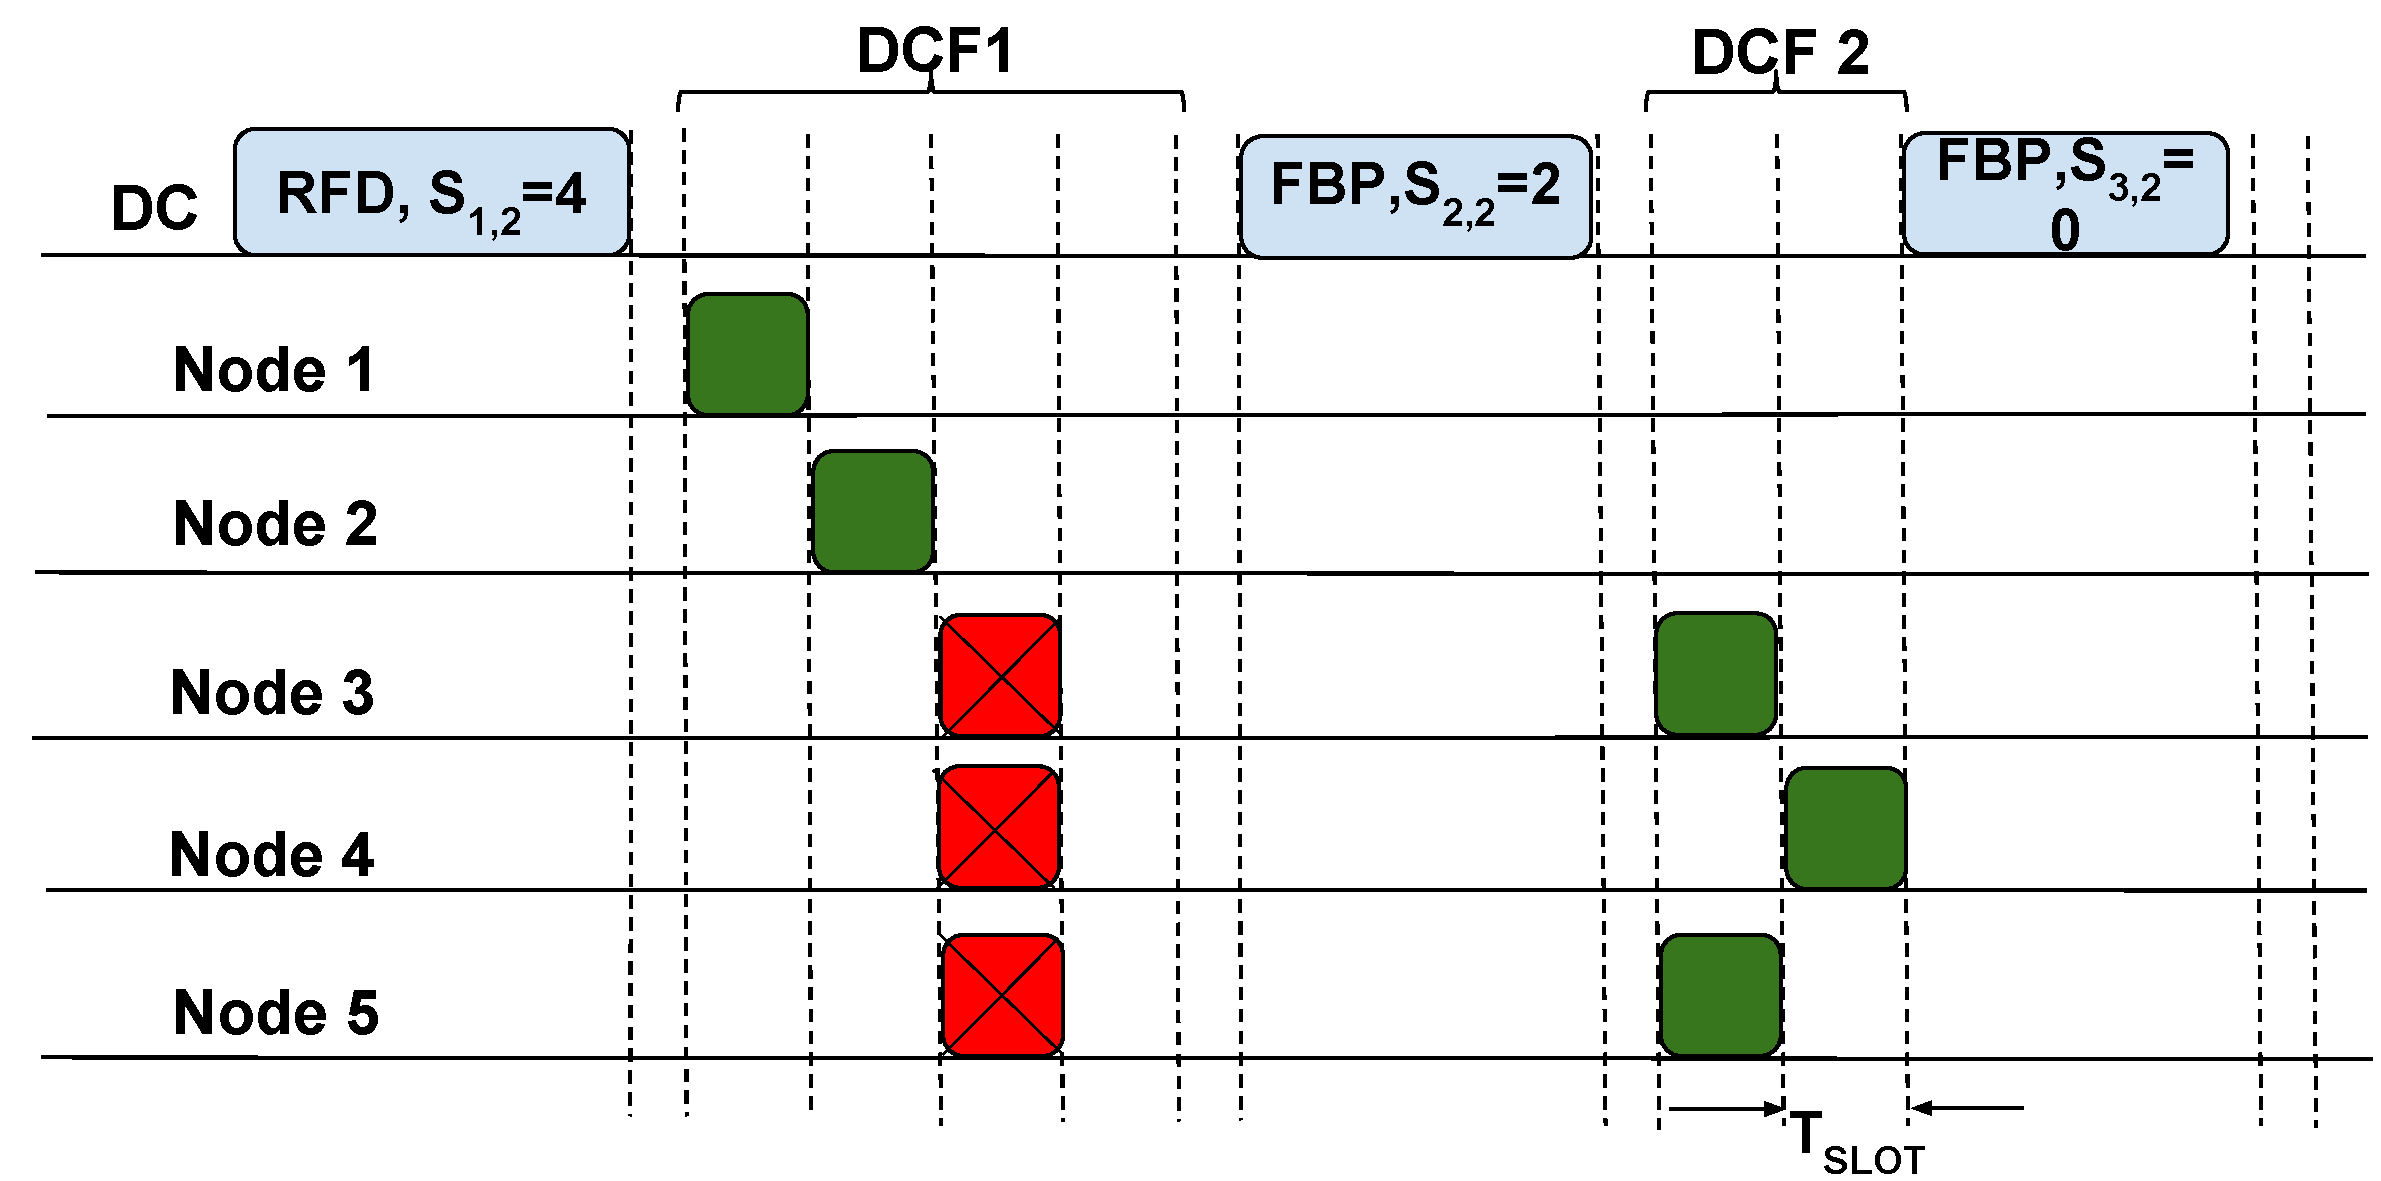
\includegraphics[width=\columnwidth]{MPR_DFSA_K2_002.pdf}
  \caption{The working of MPR-DFSA MAC Protocol with a DC having MPR threshold 2. Initially, there are five nodes in DC with one data packet each. The DC sends RFD with an initial number of slots. During the first DCF, nodes 1 and 2 become successful. During the second DCF, nodes 3,4 and 5 emerge successfully. In the second DCF, nodes 3 and 5 transmit in the same slot, but owing to the MPR threshold 2 of the DC, they become successful. The DCR ends after two DCFs.}\label{FigMPRDFSA}
\end{figure}
 Each node selects a slot randomly from the DCF. It then transmits the data in that slot.  A data transmission that takes place in a slot can have four possible outcomes namely 1) Idle - when none of the nodes transmits in that slot, 2) Collision - when $ (\textgreater K ) $ nodes transmit in that slot, 3) Success - when $ (\leq K ) $ nodes transmit in that slot and the packet is not corrupted and 4) packet corruption occurs. A feedback packet (\ac{fbp} follows every DCF that has (i) the outcome of all the slots in the previous DCF, and (ii) Number of slots in the following DCF. 
 Nodes stop contending further if they become successful. However, they listen to the FBP to know when the DCR ends.
 


  When the data is successfully transmitted to DC from all the nodes, a DCR gets completed. Once a DCR is finished, the nodes switches to sleep mode by setting up their timers until the next DCR begins. 
 Once the sleep mode gets completed, all nodes wake up synchronously and waits for the occurrence of the RFD packet(which indicates the beginning of the following DCR )sent by the DC.

 In reality, new nodes may join, or existing nodes may leave the M2M data collection network during a DCR. The dynamic variation of the number of nodes can be handled as follows. A new node has to wait and be in listen mode continuously until it hears the first RFD and then joins the DCR. If nodes leave during a DCR, the DC will have incorrect knowledge of remaining nodes ($N_{i,K}$). However, this is not a problem since a DCF with only idle or successful slots indicates the end of a DCR. 

 
  \begin{figure}[h!]
  \centering
      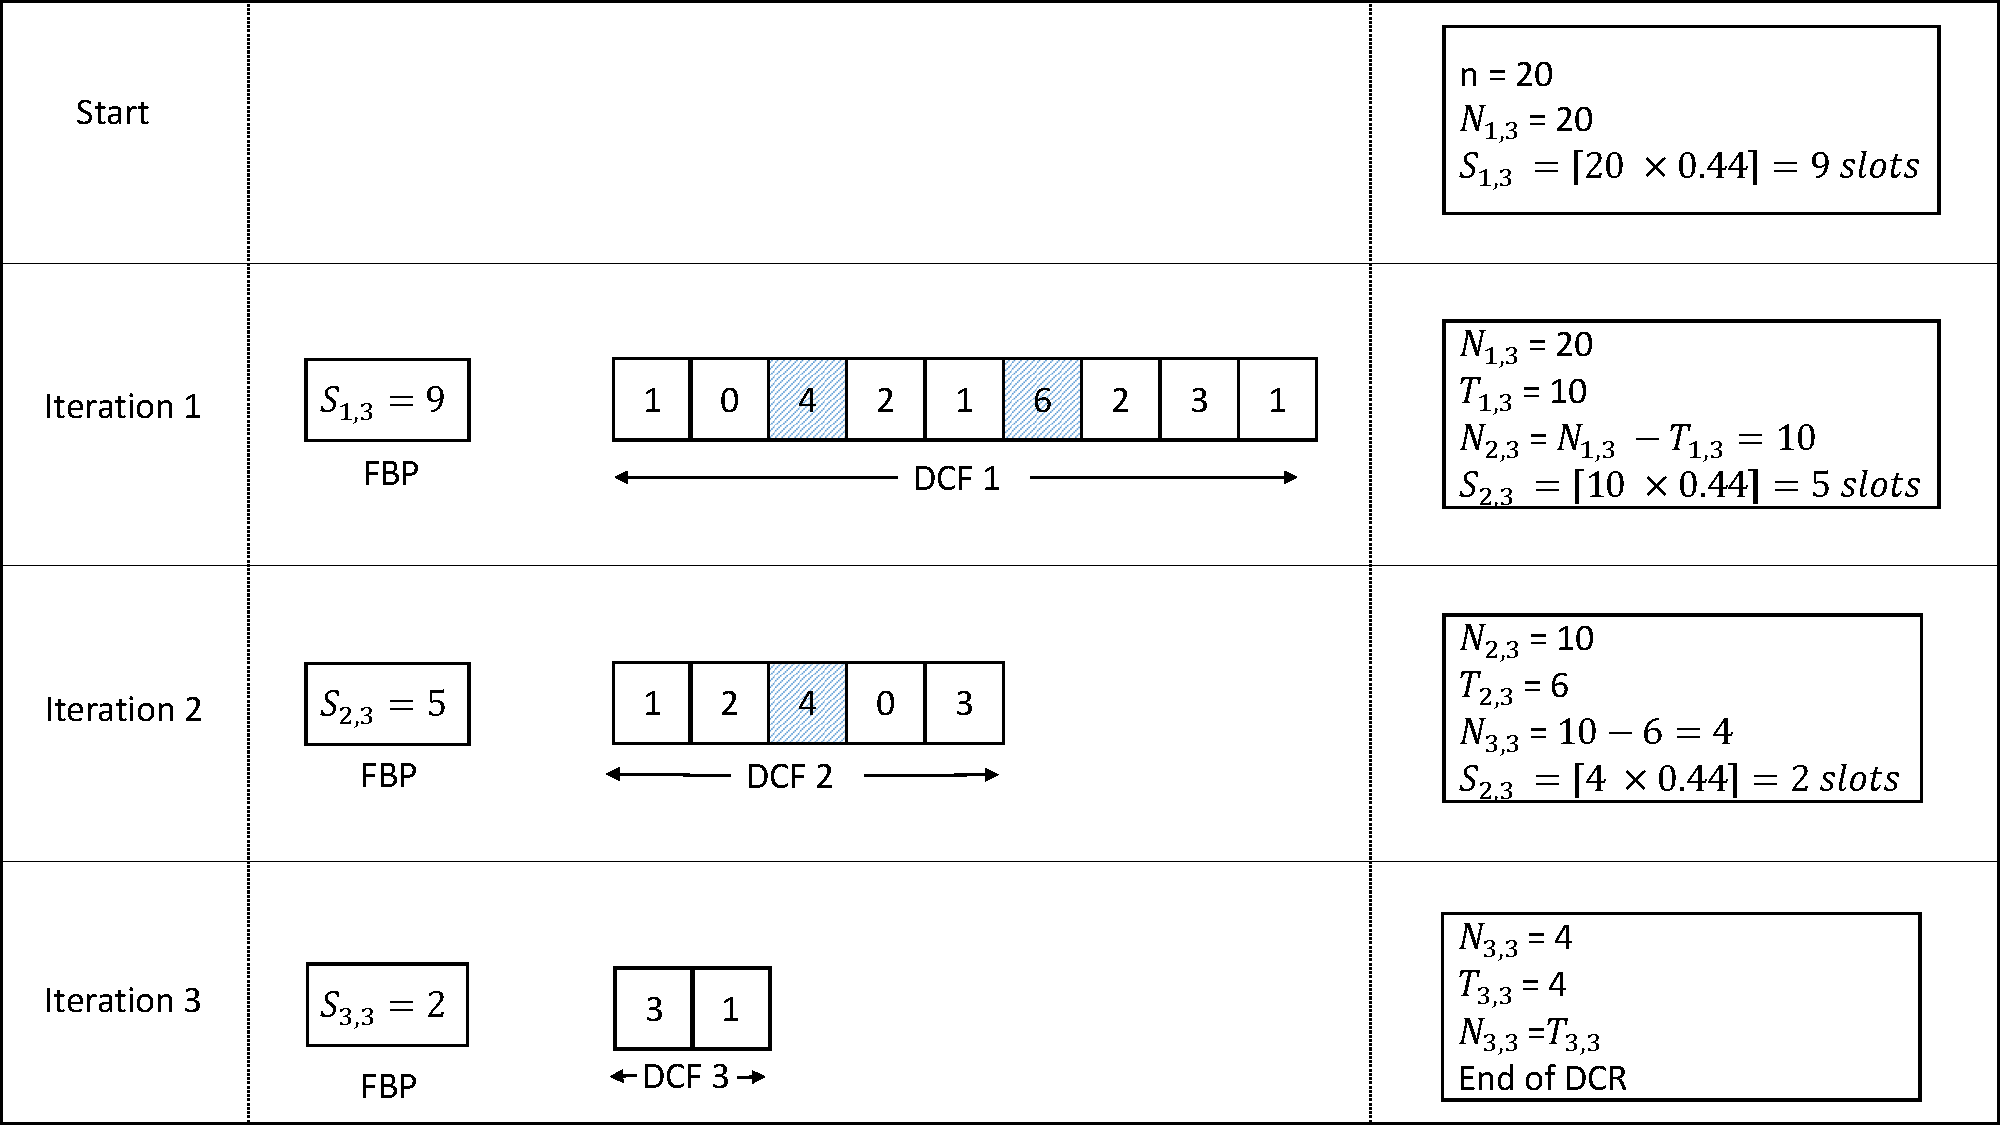
\includegraphics[width=\columnwidth]{seq_dia.pdf}
  \caption{
Sequence Diagram illustrating working of MPR DFSA algorithm. $n$ =20, $K$ = 3. $N_{i,k}$,$T_{i,k}$, and   $S_{i,k}$ are given for three iterations.DCF1 has 9 slots.Number within a slot indicate number of transmitted packets. Shaded slots indicate collision. } \label{Fig:seq}
\end{figure}